\documentclass[12pt, oneside, listof=totoc,dvipsnames]{scrbook}
\usepackage{graphicx} % Required for inserting images
\usepackage{tikz}
\usepackage{braket}
\usepackage{amsmath}
\usepackage{xcolor}
\usepackage{amssymb}
\usepackage{amsthm}
\usepackage{amsfonts}
\usepackage{float}
\usepackage{subcaption}

\usepackage{graphicx}
\usepackage[margin=1.4cm]{geometry}
\usepackage[T1]{fontenc}
\usepackage{tgbonum}
\begin{document}
	
	
	
	\newcommand{\op}[1]{\hat{#1}}
	\newcommand{\tr}[1]{T\ #1 \ T^{-1}}
	
	\vspace*{10cm}
	\begin{center}
		\Huge \textbf{Topological Insulators Notes}
	\end{center}
	\tableofcontents
	\begin{chapter}{Berry Phase}
		\section{Introduction}
		We consider a general time dependent Hamiltonian in the parameter space $H(R)$ where $R=(R_1, R_2, \ldots)$ is the vector of parameters. Suppose we want to adiabatically evolve a state in the parameter space along a curve $\mathcal{C}$, such that the variation in the parameters is done very slowly.\\
		Let $\{\ket{n(R)}\}_n$ denote an orthonormal eigenbasis of $H(R)$. Then, 
		$$H(R)\ket{n(R)}= E_n(R)\ket{n(R)}$$
		Let the system be prepared in the initial eigenstate $\ket{n(R(t=0))}$. We see how this state changes with $R(t)$ along the curve $\mathcal{C}$ in the parameter space.
		\\[0.4cm]
		In general, $\ket{n(R(t))}$ can have a time independent phase $e^{-i\theta(t)}$. Then, according to the adiabatic theorem, $$\ket{\psi(t)}=e^{-i\theta(t)}\ket{n(R(t))}$$
		This must satisfy the Schrodinger Equation.
		\begin{align*}
			&H(R)\ket{\psi(t)}=i\hbar \frac{\partial}{\partial t}\ket{\psi(t)}\\
			\implies \ &e^{-i\theta(t)}E_n \ket{n(R(t))} = i\hbar \left (-i e^{-i\theta (t)} \ket{n(R(t))}\frac{d\theta (t)}{dt}+ e^{-i\theta (t)} \frac{d}{dt}\ket{n(R(t))} \right)\\
			\implies \ & \left(E_n - \hbar \frac{d\theta}{dt}\right)\ket{n(R(t))} = i\hbar \frac{d}{dt}\ket{n(R(t))}
		\end{align*}
		Taking inner product with $\ket{n(R(t))}$ both sides, we get:
		\begin{align*}
			& \frac{d\theta}{dt} = \left( \frac{E_n}{\hbar} -i \Braket{n(R(t))|\frac{d}{dt}|n(R(t))}\right)\\
			\implies \ &\theta = \underbrace{\int \limits_0^t \frac{E_n}
				{\hbar}dt'}_{\text{Dynamic Phase}} - i \underbrace{\int \limits_0^t \Braket{n(R(t'))|\frac{d}{dt'}|n(R(t'))} dt' }_{\text{Geometric Phase}}
		\end{align*}
		Thus we get that the time dependent phase $\theta$ contains not only the usual dynamic phase but also the geometric phase. \\[0.2cm]
		Now consider the vector $ \Ket{n(R(t'))}$ in the parameter space. 
		Then, 
		\[\frac{d}{dt'}\Ket{n(R(t'))}= \sum \limits_i \left(\frac{\partial }{\partial R_i}\Ket{n(R(t'))}\right )\frac{dR_i}{dt'} = \overrightarrow{\triangledown}_R \Ket{n(R(t'))}. \frac{d\vec{R}}{dt'}\]
		
		
		
		
		Substituting it in the integral, we get:
		
		
		\begin{align*}
			&\gamma =   i \int \limits_0^t \Braket{n(R)|\overrightarrow{\triangledown}_R |n(R)}. \frac{d\vec{R}}{dt'}dt'=
			i \int \limits_\mathcal{C} \Braket{n(R)|\overrightarrow{\triangledown}_R |n(R)}. d\vec{R}
		\end{align*}
		
		Thus, we define the Berry Phase over a closed curve $\mathcal{C}$ in the parameter space as:
		\[ \boxed{\gamma_n=i \int \limits_\mathcal{C} \Braket{n(R)|\overrightarrow{\triangledown}_R |n(R)}. d\vec{R}}\]
		
		
		In analogy with the vector potential, we define the Berry Connection: $$\vec{A}_n=\Braket{n(R)|\overrightarrow{\triangledown}_R |n(R)}$$
		Then we can write $\gamma_n = \int \limits_C \vec{A}_n.d\vec{R}$
		The Berry Connection is gauge dependent. If we let $\ket{n(R)}\rightarrow e^{i\zeta(R)} \ket{n(R)}$, then $A \rightarrow A-\frac{\partial \zeta(R)}{\partial R}$. Thus, the berry phase changes by $-\int \limits_C \frac{\partial \zeta(R)}{\partial R} . dR = \zeta(R_0)-\zeta(R_T) $ where T is the long time after path C is completed in the parameter space. In general, $\zeta(R_0)\neq \zeta(R_T)$. Instead, $\zeta(R_0)- \zeta(R_T)= 2\pi m $ for some m.
		
		
		
		\begin{center}
			
			
			\tikzset{every picture/.style={line width=0.75pt}} %set default line width to 0.75pt        
			
			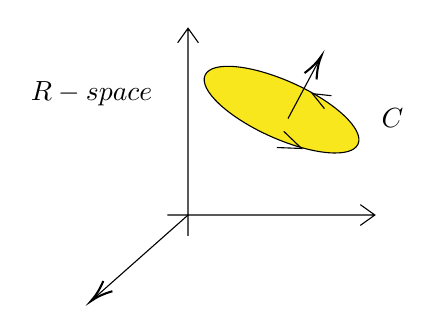
\begin{tikzpicture}[x=0.75pt,y=0.75pt,yscale=-1,xscale=1]
				%uncomment if require: \path (0,300); %set diagram left start at 0, and has height of 300
				
				%Shape: Axis 2D [id:dp3619276846946482] 
				\draw  (182,172.5) -- (282,172.5)(192,82.5) -- (192,182.5) (275,167.5) -- (282,172.5) -- (275,177.5) (187,89.5) -- (192,82.5) -- (197,89.5)  ;
				%Straight Lines [id:da43785357502108746] 
				\draw    (192,172.5) -- (146.66,212.67) ;
				\draw [shift={(145.17,214)}, rotate = 318.46] [color={rgb, 255:red, 0; green, 0; blue, 0 }  ][line width=0.75]    (10.93,-3.29) .. controls (6.95,-1.4) and (3.31,-0.3) .. (0,0) .. controls (3.31,0.3) and (6.95,1.4) .. (10.93,3.29)   ;
				%Shape: Ellipse [id:dp12830955895327378] 
				\draw  [fill={rgb, 255:red, 248; green, 231; blue, 28 }  ,fill opacity=1 ] (200.21,105.11) .. controls (203.37,98.12) and (222.41,99.9) .. (242.75,109.07) .. controls (263.1,118.25) and (277.03,131.35) .. (273.88,138.34) .. controls (270.72,145.33) and (251.68,143.56) .. (231.34,134.39) .. controls (210.99,125.21) and (197.06,112.1) .. (200.21,105.11) -- cycle ;
				%Straight Lines [id:da2994382797389161] 
				\draw    (240.17,126) -- (255.23,97.76) ;
				\draw [shift={(256.17,96)}, rotate = 118.07] [color={rgb, 255:red, 0; green, 0; blue, 0 }  ][line width=0.75]    (10.93,-3.29) .. controls (6.95,-1.4) and (3.31,-0.3) .. (0,0) .. controls (3.31,0.3) and (6.95,1.4) .. (10.93,3.29)   ;
				\draw   (257.7,121.21) -- (251.91,114.02) -- (261.09,115.01) ;
				\draw   (238.1,132.16) -- (246.72,140.43) -- (234.78,139.98) ;
				
				% Text Node
				\draw (115,106.9) node [anchor=north west][inner sep=0.75pt]    {$R-space$};
				% Text Node
				\draw (284,119.9) node [anchor=north west][inner sep=0.75pt]    {$C$};
				
				
			\end{tikzpicture}
			
		\end{center}
		
		
		We can also define a berry curvature from the berry phase.
		\begin{align*}
			\gamma_n &=i \int \limits_C \Braket{n(R)|\triangledown_R| n(R)}. d\overrightarrow{R}\\
			&= i\int \limits_C\overrightarrow{\triangledown} \times \Braket{n(R)|\triangledown_R| n(R)}. d\vec{s}&&(\text{From Stokes' Theorem})\\
			&= i \int \limits_S d\overrightarrow{s}. \underbrace{\Braket{\triangledown n(R)|\times | \triangledown n(R)}}_{\text{\textcolor{red}{Berry Curvature}}} 
		\end{align*}
		
		\section{Example: Spin in a Magnetic Field}
		The Hamiltonian for a particle with spin in a magnetic field with constant magnitude B, is: 
		$$H= - \overrightarrow{B}.\overrightarrow{\sigma}+B$$
		where $\overrightarrow{\sigma} $ is the vector of Pauli Matrices.
		Thus, 
		\[ H = \begin{pmatrix}
			B-B_z & -B_x+iB_y \\ -B_x -iB_y & B+B_z
		\end{pmatrix} \]
		Calculating the eigenvalues of H, we get $\lambda=0, 2B$. Thus, if we have two eigenstates: $\ket{\downarrow}$ and $\ket{\uparrow}$, $H\ket{\downarrow} = 0, H \ket{\uparrow}=2B\ket{\uparrow}$
		Now, since B is constant, we can use spherical coordinates to describe $\vec{B}$. 
		$$\overrightarrow{B} = \begin{pmatrix}
			B\sin \theta \cos \phi \\
			B\sin \theta \sin \phi \\
			B \cos \theta
		\end{pmatrix}$$
		Then, 
		
		\[ H = -B \begin{pmatrix}
			\cos \theta -1 & e^{-i\phi}\sin \theta \\
			e^{i\phi}\sin \theta & -\cos\theta-1
		\end{pmatrix} \]
		
		\[\ket{\downarrow} = \begin{pmatrix}
			e^{-i\phi}\sin\frac{\theta}{2} \\ -\cos \frac{\theta}{2}
		\end{pmatrix} \ \ \ket{\uparrow} = \begin{pmatrix}
			e^{-i\phi}\cos\frac{\theta}{2} \\ -\sin \frac{\theta}{2}
		\end{pmatrix}
		\]
		If we consider our parameter space as the space of $\theta$ and $\phi$, then 
		
		\begin{align*}
			A_\theta = -i \Braket{ \downarrow |\partial_\theta |\downarrow}=0\\
			A_\phi = -i \Braket{\downarrow |\partial_\phi |\downarrow}= -\sin^2 \frac{\theta}{2}
		\end{align*}
		Then, $F_{\theta\phi}= \partial_\theta A_\phi-\partial_\phi A_\theta = -\sin\theta$
		\[\int \limits_0^{2\pi}\int\limits_0^\pi F_{\theta\phi}\  d\theta d\phi= \int \limits_0^{2\pi}\int\limits_0^\pi -\sin\theta\  d\theta d\phi = 2\pi \cos\theta \Biggr|_0^\pi=-4\pi\]
		We then calculate the Berry Phase:
		\begin{align*}
			i\gamma_S= -i \int\limits_S F{ij} dS^{ij}
		\end{align*}
		\textcolor{red}{somewhere error is there\ldots correct it}
		
		\section{Experimental determination of Berry Phase}
		If we prepare two beams of particles identically and let one of the beams pass through a magnetic field which is constant throughout and another through a field which is constant in magnitude but changes direction, follow a closed loop. Then, after passing though this region, we combine the beams together. Since the second beam now has an added phase $\theta$ which is the berry phase (note that the dynamical phase is the same since it depends only on magnitude of magnetic field B), the beams will produce diffraction pattern. From this pattern, we can obtain the value of $\theta$ 
	\end{chapter}
	
	
	
	
	
	
	
	
	
	
	
	
	
	
	
	
	
	
	\begin{chapter}{Time Reversal}
		The time reversal operator $T$ is defined to be such that it reverses the arrow of time. 
		$$T: t \mapsto -t$$
		We say that, for spinless particles, T leaves $\hat{x}$ unchanged but changes $\hat{p}$. This can be thought of because $T$ reverses the arrow of time, thus $\hat{p}$ which is related to the `velocity' (which is time dependent), is also reversed. 
		\begin{align*}
			T\ \hat{x}\ T^{-1}&=\hat{x}\\
			T\ \hat{p}\ T^{-1}&=-\hat{p}
		\end{align*}
		
		\begin{align*}
			T\ i \hbar \ T^{-1}&= T\ [\hat{x}, \hat{p}]\ T^{-1}\\
			&=T \ (\op{x}\op{p}- \op{p}\op{x}) \ T^{-1}\\
			&= T\  \op{x}\op{p}\ T^{-1}- T \ \op{p}\op{x} \ T^{-1}\\
			&= T\  \op{x}\ \mathbb{I}\ \op{p}\ T^{-1}- T \ \op{p}\ \mathbb{I}\ \op{x} \ T^{-1}\\
			&= T\  \op{x}\ T^{-1} T\ \op{p}\ T^{-1}- T \ \op{p}\  T^{-1}T \ \op{x} \ T^{-1}\\
			&= \op{x} \ T\ \op{p}\ T^{-1}+\op{p} \ T\ \op{x} \ T^{-1}\\
			&= -\op{x}\op{p}+\op{p} \op{x}\\
			&=-[\op{x},\op{p}]\\
			&= -i\hbar
		\end{align*}
		Since $\hbar$ is a scalar constant, we can say that $$\boxed{T \ i \ T^{-1} = -i}$$ That is, $T$ acts as the complex conjugation operator $K$. 
		
		In general, $T$ can be written as :$$T=UK$$ where U is an unitary operator, that is, $U U^\dagger = \mathbb{I}$.\\[0.2cm]
		Note that: $K^2=\mathbb{I}$ since taking complex conjugation twice returns to original value. Then from this, $K^{-1}=K$\\[0.2cm]
		\noindent
		With this general definition, we now show that the anti-unitary property is also satisfied.
		\begin{align*}
			UK \ i \ (UK)^{-1} &= U K \ i \ K^{-1} U^{-1}\\
			&=  U (-i) U^{-1}\\
			&=-i U  U^{-1}\\
			&= -i \\
		\end{align*}
		We note the following results:
		\begin{itemize}
			\item $$KU=U^* \implies KUK= U^*K$$
			\item 
			\begin{align*}
				& U U^\dagger = \mathbb{I}\\ \implies
				& U (U^*)^T =  \mathbb{I}\\\implies
				& KU (U^*)^T = K \mathbb{I} =\mathbb{I}\\\implies
				& KU =  ((U^*)^T) ^{-1}\\\implies
				&KUK =  ((U^*)^T) ^{-1}K\\\implies
			\end{align*}
		\end{itemize}
		
		
		
		We now investigate the action of $T^2$ where $T$ takes the previous general form.
		\begin{align*} 
			T^2 &= UKUK\\
			&= U (KUK)\\
			&= U U^*\\
			&= U (U^T)^{-1}
		\end{align*}
		Intuitively, we can say that the action of $T^2$ should return a system to its original state (upto a phase factor). 
		Thus, $T^2= \phi $, where $\phi$ is a diagonal matrix consisting of phases. 
		\noindent
		Hence, we can say that: 
		\begin{align*}
			&U (U^T)^{-1}=\phi \\
			\implies &U= \phi \ U^T
		\end{align*}
		Taking transpose both sides, we get:
		$U^T=U\phi $ (since $\phi$ is a diagonal matrix, $\phi^T=\phi$)
		From these two equations, we get:
		$$U=\phi \ U \ \phi$$
		From this fact, we can say that $\phi = \pm
		\mathbb{I}$. Thus, 
		$$\boxed{T^2= \pm \mathbb{I}}$$
		A system is said to have time reversal symmetry is the Hamiltonian of the system commutes with $T$, that is, $[H,T]=0$
		
		\begin{center}
			\Large  \textcolor{blue}{Spinless Particle}
		\end{center}
		
		\section{Time Reversal in Lattice for Spinless Particles}
		
		Similar to our analogy of $T$ keeping $\op{x}$ invariant, we define that $T$ keeps the creation/annihilation operators invariant.
		$$T\ \op{c}_j \ T^{-1} = \op{c}_j$$ We now investigate the action of $T$ on the creation operator in momentum space $\op{c}_k$.
		We know, 
		\begin{align*}
			&\op{c}_k = \frac{1}{\sqrt{N}}\sum \limits_j e^{-ijR_j}\op{c}_j
		\end{align*}
		
		\begin{align*}
			T \ c_k \ T^{-1} &= \frac{1}{\sqrt{N}}\sum \limits_j e^{ijR_j}\ T\ \op{c}_j T^{-1}\  &&\text{(since T changes i to -i)}\\
			&=\frac{1}{\sqrt{N}}\sum \limits_j e^{ijR_j}\op{c}_j\\
			&=\frac{1}{\sqrt{N}}\sum \limits_j e^{-i(-j)R_j}\op{c}_{-j}\\
			&=c_{-k}
		\end{align*}
		Thus, we have: 
		$$\boxed{ T \ c_k \ T^{-1}= c_{-k}}$$
		\noindent
		Any Hamiltonian which is translationally invariant can be written as $$H= \sum \limits_k c^\dagger_k \ h(k) \ c_k$$
		Then,
		
		\begin{align*}
			T \ H \ T^{-1}&=  \sum \limits_k  \tr{(\ c^\dagger_k \ h(k)\  c_k}\\
			&=  \sum \limits_k  \tr{(\ c^\dagger_k \ \mathbb{I}\ h(k)\ \mathbb{I}\ c_k)}\\
			&=\sum \limits_k  \tr{c^\dagger_k}\tr{h(k)}\tr{c_k}\\
			&=\sum \limits_k  (\tr{c^\dagger_k})(\tr{h(k)})(\tr{c_k})\\
			&=\sum \limits_k  c^\dagger_{-k}\ (\tr{h(k)})\ c_{-k}
		\end{align*}
		If the system is to possess time reversal symmetry, then $T \ H \ T^{-1} = H$. From this, we can say by comparison that: 
		$$\boxed{\tr{h(k)}=h(-k)}$$
		\noindent
		If $\psi(k)$ is an eigenstate of $h(k)$, then :
		\begin{align*}
			h(k)\psi(k)&=E_k\psi(k)\\
			T \ h(k) \psi(k) &= E_k \ T \ \psi(k) && (\text{As $E_k$ is real, T has no effect})\\
			T \ h(k) \ T^{-1}T \ \psi(k) &= E_k \ T \ \psi(k) \\
			h(-k) \ T\psi(k) &= E_k \ T \ \psi(k) 
		\end{align*}
		Thus, we see that $T\psi(k)$ is an eigenstate of $h(-k)$
		\noindent
		\begin{center}
			\fbox{If $\psi(k)$ is an eigenstate of $h(k)$, then $T\psi(k)$ is an eigenstate of $h(-k)$ }
		\end{center}
		
		
		
		
		
		
		\section{Vanishing of Hall Conductance for Time Reversal Symmetry}
		For a state $\ket{u(k)}=(u_1, u_2, \ldots)$, we  know the Berry Curvature: $F_{ij}(k) = -i\braket{\partial_i u(k)|\partial_j u(k)}$.
		Then,
		\begin{align*}
			F_{ij}(-k) &= -i\braket{\partial_i u(-k)|\partial_j u(-k)}\\
			&= -i\sum \limits_m \partial_i u_m(-k)^* \partial_j u_m(-k)\\
			&= -i\sum \limits_m \partial_i u_m(k) \partial_j u_m^*(k)\\
			&=F_{ij}(k)
		\end{align*}
		
		\noindent
		Since we get $F_{ij}(-k) = F_{ij}(k)$, we say that in systems having TR Symmetry, the berry curvature is an odd function. Hence, its integral over the BZ must be 0. 
		Since $$ \int \limits_S F_{ij} dS^{ij} = 2\pi C$$ we have that $C=0$. Since the Hall conductivity $\sigma_{xy}$ is related to the Chern Number, we conclude that $\sigma_{xy}$ is also zero. Thus, the Hall conductance vanishes in presence of TR Symmetry.
		
		\begin{center}
			\Large  \textcolor{blue}{Spinful Particle}\\
			
		\end{center}
		\noindent
		We now consider the spin degree of freedom too. Consider particles with spin $\mathbf{S}$. Since we can intuitively say that angular momentum is a kind of `momentum', thus: $$\mathcal{T} \ \mathbf{S}\  \mathcal{T}^{-1} = -\mathbf{S}$$ Thus, spins flip under time reversal operation by an angle $\pi$. By convention, we consider this rotation to be around the Y-axis. Thus, the general form of $\mathcal{T}= e^{-i\pi S_y}K$\\[0.2cm]
		We now find the action of $\mathcal{T}^2.$
		\begin{align*}
			\mathcal{T}^2 &=e^{-i\pi S_y}K\ e^{-i\pi S_y}K\\
			&=e^{-i\pi S_y}K\ e^{-i\pi S_y}K^{-1} &&(\text{as $K=K^{-1}$})\\
			&=e^{-i\pi S_y}e^{i\pi S^*_y}\\
			&=e^{-i\pi (S_y-S^*_y)}
		\end{align*}
		We can choose an arbitrary basis in which $S_y$ is purely imaginary. Let $S_y= i\Tilde{S_y}$ where $\Tilde{S_y}$ is real. Then, $S^*_y= -i\Tilde{S_y}$. Thus, $$S_y-S^*_y =  i\Tilde{S_y}+ i\Tilde{S_y}=2 i\Tilde{S_y}=2S_y$$
		Hence,  $$ \boxed{\mathcal{T}^2 = e^{-2i\pi S_y}}$$
		
		\begin{itemize}
			\item \textcolor{red}{For integer spin:} $\mathcal{T}^2 =\mathbb{I}$ 
			\item \textcolor{red}{For half-integer spin:} $\mathcal{T}^2 =-\mathbb{I}$ 
		\end{itemize}
		\section{Kramers' Theorem}
		\textbf{For each energy in a system with particles having half-integer spin, there are atleast two degenerate states.}\\[0.3cm]
		\textit{Proof:} Let $\ket{\psi}$ be an eigenstate of a TR Symmetric hamiltonian H with energy E. As previously proved, 
		$T^2=-\mathbb{I}$ for half-integer spins. Thus, $T^2=UU^*=-1$\\[0.2cm]
		Also,  $$U(U^*)^T=1 \implies (U^*)^T=U^{-1}\implies U^*=(U^{-1})^T=(U^{T})^{-1} $$Putting this in previous equation, we get: 
		$$-1=UU^*=U(U^{T})^{-1} \implies U=-U^T$$
		\noindent
		Note that: \begin{align*}
			HT\ket{\psi} = TH\ket{\psi}=TE\ket{\psi}=ET\ket{\psi}
		\end{align*}
		Hence $T\ket{\psi}$ is also an eigenstate of H.
		Also,
		\begin{align*}
			\Braket{\psi|T\psi} &= \sum \limits_{m,n} \psi^*_m U_{mn}K \psi_n \\
			&=\sum \limits_{m,n} \psi^*_m U_{mn} \psi^*_n\\
			&= - \sum \limits_{m,n} \psi^*_m U_{nm} \psi^*_n\\
			&=- \Braket{\psi|T\psi}\\
			&\implies \Braket{\psi|T\psi}=0 
		\end{align*}
		Thus, $\ket{\psi}$ and $\ket{T\psi}$ are orthogonal to each other and have same eigenvalue E. Thus, these are degenerate states. 
		
		
		
		\section{Time Reversal in Lattice for Spinful Particles}
		We consider the case of half-integer spins. As before the Hamiltonian after Fourier Transform can be written as:
		\[H= \sum \limits_\mathbf{k} c^\dagger_{\mathbf{k}\alpha\sigma}h^{\sigma,\sigma'}_{\alpha,\beta}(\mathbf{k})c_{\mathbf{k}\beta\sigma'}\]
		$\alpha, \beta$: orbital indices\\
		$\sigma, \sigma'$: spin indices\\
		
		\noindent
		We want to see how TR acts on the operators $c_{ja\sigma}$ and $c^\dagger_{ja\sigma}$. For this, we first see action of $Tc_\uparrow$ on state $c^\dagger_\uparrow \ket{0}$ which is singly-occupied.\\[0.4cm]
		\textcolor{blue}{Note: Since we know that TR flips spin, we can write: \begin{align*}
				Tc_\downarrow T^{-1}=Ac_\uparrow \hspace{1cm}  Tc_\uparrow T^{-1}=Bc_\downarrow  
			\end{align*} where A,B are phases to be determined.}
		\vspace*{1cm}
		\begin{align*}
			Tc_\uparrow c^\dagger_\uparrow \ket{0} &= T \ket{0} = \ket{0}^* \\ Tc_\uparrow c^\dagger_\uparrow \ket{0} &= Bc_\downarrow T c^\dagger_\uparrow \ket{0}\\ 
			&=B T^{-1} T c_\downarrow T c^\dagger_\uparrow \ket{0}\\
			&=B T^{-1}A c_\uparrow T T c^\dagger_\uparrow \ket{0}\\
			&=B T^{-1}A c_\uparrow T^2 (c^\dagger_\uparrow \ket{0})\\
			&=-AB T^{-1} c_\uparrow (c^\dagger_\uparrow \ket{0}) &&(\text{Since } c^\dagger_\uparrow \ket{0} \text{is a singly occupied site})\\
			&=-AB T^{-1}\ket{0}\\
			&=-ABT\ket{0} (\text{Since } \ket{0} \text{is 0 (even) occupancy})\\
			&=-AB\ket{0}^*
		\end{align*}
		From the above two relations, we get $AB=-1$. Thus, if we choose $A=-1$, we have $B=1$. Generalising this, we write: 
		\begin{align*}
			\boxed{ Tc_{ja\downarrow} T^{-1}=-c_{ja\uparrow} \hspace{1cm}  Tc_{ja\uparrow} T^{-1}=c_{ja\downarrow } }
		\end{align*} 
		As in the case of spinless particles, we now see how TR acts on the Bloch hamiltonian. For this, we perform fourier transform. We know: 
		\[c_{ja\sigma}=\frac{1}{\sqrt{N}} \sum \limits_\mathbf{k}e^{i\mathbf{k.R_j}}c_{ka\sigma} \implies c_{ka\sigma}=\frac{1}{\sqrt{N}} \sum \limits_\mathbf{k}e^{-i\mathbf{k.R_j}}c_{ja\sigma} \]
		\begin{align*}
			T \ c_{ka\sigma}\ T^{-1}= \frac{1}{\sqrt{N}} \sum \limits_\mathbf{k}e^{+i\mathbf{k.R_j}}\ T\ c_{ja\sigma} \ T^{-1}\\
			&=
		\end{align*}
	\end{chapter}
	
	
	
	
	
	
	
	
	
	
	
	
	
	
	
	
	
	
	
	
	
	\begin{chapter}{Magnetic Field on a Square Lattice}
		
		We analyse a tight binding hamiltonian for a 2D lattice when a magnetic field is applied. The Hamiltonian can be written in terms of translation operators in the x and y directions. 
		\[H= T_x+T_y+T^\dagger_x+T^\dagger_y\]
		\noindent
		The translation operators take the form:
		\[T_x = \sum \limits_{m,n} c^\dagger_{m+1,n}c_{m,n}e^{i\theta^x_{m,n}} \ \ T_y = \sum \limits_{m,n} c^\dagger_{m,n+1}c_{m,n}e^{i\theta^y_{m,n}}\]
		\noindent
		Since we are considering only nearest neighbour hopping, we can write: \textcolor{blue}{this is due to pierls substitution\ldots write about it}
		\begin{align*}
			\theta^x_{m,n} = \frac{e}{\hbar}\int \limits_m^{m+1} \Vec{A}. d\Vec{x}\hspace{1cm}
			\theta^y_{m,n} = \frac{e}{\hbar}\int \limits_n^{n+1} \Vec{A}. d\Vec{y}
		\end{align*}
		
		With analogy from continuous derivatives, define lattice derivative: 
		\begin{align*}
			\triangle_x f_{mn} = f_{m+1,n}-f_{m,n}\hspace{1cm}
			\triangle_y f_{mn} = f_{m,n+1}-f_{m,n}
		\end{align*}
		
		
		
		
		\begin{center}
			
			
			
			
			\tikzset{every picture/.style={line width=0.75pt}} %set default line width to 0.75pt        
			
			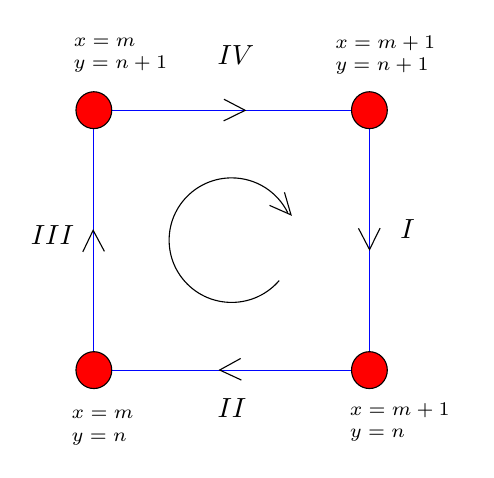
\begin{tikzpicture}[x=0.75pt,y=0.75pt,yscale=-1,xscale=1]
				%uncomment if require: \path (0,300); %set diagram left start at 0, and has height of 300
				
				%Shape: Rectangle [id:dp6851066124620712] 
				\draw  [color={rgb, 255:red, 0; green, 5; blue, 255 }  ,draw opacity=1 ] (98.62,117.88) -- (231.38,117.88) -- (231.38,243.12) -- (98.62,243.12) -- cycle ;
				%Shape: Ellipse [id:dp37147423069411123] 
				\draw  [fill={rgb, 255:red, 255; green, 0; blue, 0 }  ,fill opacity=1 ] (90,117.88) .. controls (90,112.98) and (93.86,109) .. (98.62,109) .. controls (103.38,109) and (107.24,112.98) .. (107.24,117.88) .. controls (107.24,122.79) and (103.38,126.76) .. (98.62,126.76) .. controls (93.86,126.76) and (90,122.79) .. (90,117.88) -- cycle ;
				%Shape: Ellipse [id:dp8434701576783272] 
				\draw  [fill={rgb, 255:red, 255; green, 0; blue, 0 }  ,fill opacity=1 ] (222.76,117.88) .. controls (222.76,112.98) and (226.62,109) .. (231.38,109) .. controls (236.14,109) and (240,112.98) .. (240,117.88) .. controls (240,122.79) and (236.14,126.76) .. (231.38,126.76) .. controls (226.62,126.76) and (222.76,122.79) .. (222.76,117.88) -- cycle ;
				%Shape: Ellipse [id:dp7898873095219001] 
				\draw  [fill={rgb, 255:red, 255; green, 0; blue, 0 }  ,fill opacity=1 ] (90,243.12) .. controls (90,238.21) and (93.86,234.24) .. (98.62,234.24) .. controls (103.38,234.24) and (107.24,238.21) .. (107.24,243.12) .. controls (107.24,248.02) and (103.38,252) .. (98.62,252) .. controls (93.86,252) and (90,248.02) .. (90,243.12) -- cycle ;
				%Shape: Ellipse [id:dp5247097453247115] 
				\draw  [fill={rgb, 255:red, 255; green, 0; blue, 0 }  ,fill opacity=1 ] (222.76,243.12) .. controls (222.76,238.21) and (226.62,234.24) .. (231.38,234.24) .. controls (236.14,234.24) and (240,238.21) .. (240,243.12) .. controls (240,248.02) and (236.14,252) .. (231.38,252) .. controls (226.62,252) and (222.76,248.02) .. (222.76,243.12) -- cycle ;
				%Shape: Arc [id:dp9197421265937379] 
				\draw  [draw opacity=0] (187.92,199.97) .. controls (182.39,206.41) and (174.18,210.5) .. (165,210.5) .. controls (148.36,210.5) and (134.88,197.07) .. (134.88,180.5) .. controls (134.88,163.93) and (148.36,150.5) .. (165,150.5) .. controls (176.87,150.5) and (187.13,157.34) .. (192.04,167.27) -- (165,180.5) -- cycle ; \draw   (187.92,199.97) .. controls (182.39,206.41) and (174.18,210.5) .. (165,210.5) .. controls (148.36,210.5) and (134.88,197.07) .. (134.88,180.5) .. controls (134.88,163.93) and (148.36,150.5) .. (165,150.5) .. controls (176.87,150.5) and (187.13,157.34) .. (192.04,167.27) ;  
				\draw   (190.45,157.45) -- (193.6,168.32) -- (183.25,163.75) ;
				\draw   (169.7,247.92) -- (159.24,243.07) -- (169.34,237.51) ;
				\draw   (161.31,112.61) -- (171.52,117.96) -- (161.17,123.04) ;
				\draw   (236.53,174.69) -- (231.44,185.03) -- (226.11,174.81) ;
				\draw   (93.29,186.15) -- (98.27,175.75) -- (103.71,185.91) ;
				
				% Text Node
				\draw (80,257.9) node [anchor=north west][inner sep=0.75pt]  [font=\scriptsize]  {$ \begin{array}{l}
						x=m\\
						y=n
					\end{array}$};
				% Text Node
				\draw (214,256.4) node [anchor=north west][inner sep=0.75pt]  [font=\scriptsize]  {$ \begin{array}{l}
						x=m+1\\
						y=n
					\end{array}$};
				% Text Node
				\draw (81,78.4) node [anchor=north west][inner sep=0.75pt]  [font=\scriptsize]  {$ \begin{array}{l}
						x=m\\
						y=n+1
					\end{array}$};
				% Text Node
				\draw (207,79.4) node [anchor=north west][inner sep=0.75pt]  [font=\scriptsize]  {$ \begin{array}{l}
						x=m+1\\
						y=n+1
					\end{array}$};
				% Text Node
				\draw (245,169.4) node [anchor=north west][inner sep=0.75pt]    {$I$};
				% Text Node
				\draw (157,255.4) node [anchor=north west][inner sep=0.75pt]    {$II$};
				% Text Node
				\draw (67,172.4) node [anchor=north west][inner sep=0.75pt]    {$III$};
				% Text Node
				\draw (157,85.4) node [anchor=north west][inner sep=0.75pt]    {$IV$};
				
				
			\end{tikzpicture}
			
			
			
			
			
			
			
		\end{center}
		\noindent
		The lattice curl of the phase factors is given by the flux per plaquette $\phi_{mn}$.
		
		\begin{align*}
			\triangle_x  \theta^y_{m,n} - \triangle_y \theta^x_{m,n} &= \theta^y_{m+1,n}- \theta^y_{m,n}- \theta^x_{m,n+1}+ \theta^x_{m,n}\\
			&= \frac{e}{\hbar}\left(\int \limits_n^{n+1} \underbrace{\Vec{A}. d\Vec{y}}_{x=m+1} - \int \limits_n^{n+1} \underbrace{\Vec{A}. d\Vec{y}}_{x=m}-\int \limits_m^{m+1} \underbrace{\Vec{A}. d\Vec{x}}_{y=n+1}+\int \limits_m^{m+1} \underbrace{\Vec{A}. d\Vec{x}}_{y=n}\right)\\
			&=\frac{e}{\hbar}\left(\int \limits_I \Vec{A}. d\Vec{l} +\int \limits_{III} \Vec{A}. d\Vec{l}+\int \limits_{IV}\Vec{A}. d\Vec{l}+\int \limits_{II} \Vec{A}. d\Vec{l}\right)\\
			&= \frac{e}{\hbar}\int \limits_{\text{plaquette}}\Vec{A}. d\Vec{l}\\
			&=\frac{2\pi e}{h}\int_S \Vec{B}.d\Vec{s}&&(\text{from Stokes' theorem})\\ 
			&=2\pi \phi_{mn}
		\end{align*}
		
		\section{Translation operators do not commute}
		Suppose our system consists of a single-particle at site (m,n). The state is then given by $\ket{\psi_{ij}}= c^\dagger_{i,j}\ket{0}$
		
		
		
		\begin{align*}
			T_xT_y\ket{\psi_{ij}} &=T_x c^\dagger_{i,j+1}e^{i\theta^y_{i,j} \ket{0}}=e^{i\theta^x_{i,j+1}}e^{i\theta^y_{i,j}}c^\dagger_{i+1,j+1} \ket{0}=e^{i(\theta^x_{i,j+1}+\theta^y_{i,j})}
			c^\dagger_{i+1,j+1} \ket{0}\\
			T_yT_x\ket{\psi_{ij}} &=T_y c^\dagger_{i+1,j}e^{i\theta^x_{i,j} \ket{0}}=e^{i\theta^y_{i+1,j}}e^{i\theta^x_{i,j}}c^\dagger_{i+1,j+1} \ket{0}\\&=e^{i(\theta^y_{i+1,j}+\theta^x_{i,j})} c^\dagger_{i+1,j+1} \ket{0}\\
			&=e^{2\pi i \phi_{mn}+i(\theta^x_{i,j+1}+\theta^y_{i,j})} c^\dagger_{i+1,j+1} \ket{0}\\
			&=e^{2\pi i \phi_{mn}}T_xT_y\ket{\psi_{ij}}
		\end{align*}
		Thus, we see that $T_x$ and $T_y$ do not commute in general and hence do not commute with the Hamiltonian (as Hamiltonian is the sum of these two operators). Thus the Hamiltonian is not translationally invariant with respect to $T_x, T_y$.
		We now define \textcolor{blue}{Magnetic Translation Operators}
		\[\op{T}_x = \sum \limits_{m,n} c^\dagger_{m+1,n}c_{m,n}e^{i\chi^x_{m,n}} \ \ \op{T}_y = \sum \limits_{m,n} c^\dagger_{m,n+1}c_{m,n}e^{i\chi^y_{m,n}}\]
		We want $[H,\op{T}_x]=0$ and $[H,\op{T}_y]=0$ which essentially means that we have to impose conditions on $\chi_{m,n}$ such that $[\op{T}_x,T_x]=0$ and $[\op{T}_x,T_y]=0$
		\begin{itemize}
			\item $[\op{T}_x,T_x]=0$ 
			\begin{align*}
				\op{T}_xT_x=T_x\op{T}_x
			\end{align*}
		\end{itemize}
	\end{chapter}
	
	
	
	
	
	
	\begin{chapter}{Graphene}
		\begin{center}
			
			
			\tikzset{every picture/.style={line width=0.75pt}} %set default line width to 0.75pt        
			
			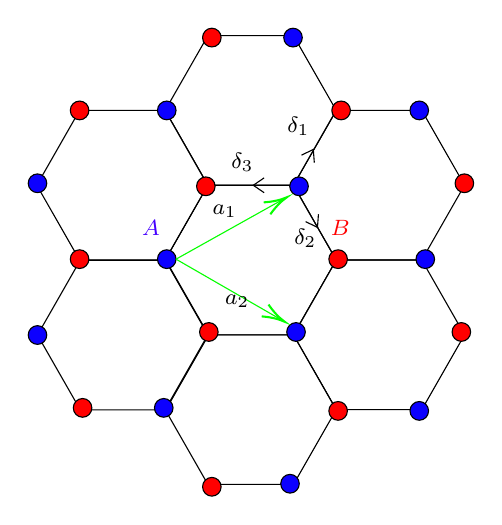
\begin{tikzpicture}[x=0.75pt,y=0.75pt,yscale=-1,xscale=1]
				%uncomment if require: \path (0,300); %set diagram left start at 0, and has height of 300
				
				%Shape: Polygon [id:dp19631241618016704] 
				\draw   (131.97,96.87) -- (111.36,132.91) -- (70.14,132.91) -- (49.53,96.87) -- (70.14,60.83) -- (111.36,60.83) -- cycle ;
				%Shape: Polygon [id:dp3462461793230377] 
				\draw   (193.8,132.91) -- (173.19,168.95) -- (131.97,168.95) -- (111.36,132.91) -- (131.97,96.87) -- (173.19,96.87) -- cycle ;
				%Shape: Polygon [id:dp6770798649040526] 
				\draw   (132.3,169.04) -- (111.69,205.08) -- (70.47,205.08) -- (49.86,169.04) -- (70.47,133) -- (111.69,133) -- cycle ;
				%Shape: Polygon [id:dp8314563030843936] 
				\draw   (193.8,204.99) -- (173.19,241.03) -- (131.97,241.03) -- (111.36,204.99) -- (131.97,168.95) -- (173.19,168.95) -- cycle ;
				%Shape: Polygon [id:dp538739529133375] 
				\draw   (255.62,168.95) -- (235.02,204.99) -- (193.8,204.99) -- (173.19,168.95) -- (193.8,132.91) -- (235.02,132.91) -- cycle ;
				%Shape: Polygon [id:dp6058058663434542] 
				\draw   (255.62,96.87) -- (235.02,132.91) -- (193.8,132.91) -- (173.19,96.87) -- (193.8,60.83) -- (235.02,60.83) -- cycle ;
				%Shape: Polygon [id:dp3815762380193616] 
				\draw   (193.8,60.83) -- (173.19,96.87) -- (131.97,96.87) -- (111.36,60.83) -- (131.97,24.79) -- (173.19,24.79) -- cycle ;
				%Shape: Ellipse [id:dp15064243727418603] 
				\draw  [fill={rgb, 255:red, 255; green, 0; blue, 0 }  ,fill opacity=1 ] (65.67,60.83) .. controls (65.67,58.34) and (67.67,56.32) .. (70.14,56.32) .. controls (72.61,56.32) and (74.61,58.34) .. (74.61,60.83) .. controls (74.61,63.32) and (72.61,65.34) .. (70.14,65.34) .. controls (67.67,65.34) and (65.67,63.32) .. (65.67,60.83) -- cycle ;
				%Shape: Ellipse [id:dp3865290801123574] 
				\draw  [fill={rgb, 255:red, 255; green, 0; blue, 0 }  ,fill opacity=1 ] (126.51,97.39) .. controls (126.51,94.9) and (128.51,92.88) .. (130.97,92.88) .. controls (133.44,92.88) and (135.44,94.9) .. (135.44,97.39) .. controls (135.44,99.88) and (133.44,101.9) .. (130.97,101.9) .. controls (128.51,101.9) and (126.51,99.88) .. (126.51,97.39) -- cycle ;
				%Shape: Ellipse [id:dp9617999550105512] 
				\draw  [fill={rgb, 255:red, 255; green, 0; blue, 0 }  ,fill opacity=1 ] (191.68,60.83) .. controls (191.68,58.34) and (193.68,56.32) .. (196.15,56.32) .. controls (198.62,56.32) and (200.62,58.34) .. (200.62,60.83) .. controls (200.62,63.32) and (198.62,65.34) .. (196.15,65.34) .. controls (193.68,65.34) and (191.68,63.32) .. (191.68,60.83) -- cycle ;
				%Shape: Ellipse [id:dp795490748883834] 
				\draw  [fill={rgb, 255:red, 255; green, 0; blue, 0 }  ,fill opacity=1 ] (65.67,132.49) .. controls (65.67,130) and (67.67,127.98) .. (70.14,127.98) .. controls (72.61,127.98) and (74.61,130) .. (74.61,132.49) .. controls (74.61,134.98) and (72.61,136.99) .. (70.14,136.99) .. controls (67.67,136.99) and (65.67,134.98) .. (65.67,132.49) -- cycle ;
				%Shape: Ellipse [id:dp057539516108925604] 
				\draw  [fill={rgb, 255:red, 255; green, 0; blue, 0 }  ,fill opacity=1 ] (251.07,95.93) .. controls (251.07,93.44) and (253.07,91.42) .. (255.53,91.42) .. controls (258,91.42) and (260,93.44) .. (260,95.93) .. controls (260,98.42) and (258,100.44) .. (255.53,100.44) .. controls (253.07,100.44) and (251.07,98.42) .. (251.07,95.93) -- cycle ;
				%Shape: Ellipse [id:dp5301512610135036] 
				\draw  [fill={rgb, 255:red, 255; green, 0; blue, 0 }  ,fill opacity=1 ] (127.95,167.58) .. controls (127.95,165.09) and (129.95,163.07) .. (132.42,163.07) .. controls (134.89,163.07) and (136.89,165.09) .. (136.89,167.58) .. controls (136.89,170.07) and (134.89,172.09) .. (132.42,172.09) .. controls (129.95,172.09) and (127.95,170.07) .. (127.95,167.58) -- cycle ;
				%Shape: Ellipse [id:dp5357788129928909] 
				\draw  [fill={rgb, 255:red, 255; green, 0; blue, 0 }  ,fill opacity=1 ] (190.24,132.49) .. controls (190.24,130) and (192.23,127.98) .. (194.7,127.98) .. controls (197.17,127.98) and (199.17,130) .. (199.17,132.49) .. controls (199.17,134.98) and (197.17,136.99) .. (194.7,136.99) .. controls (192.23,136.99) and (190.24,134.98) .. (190.24,132.49) -- cycle ;
				%Shape: Ellipse [id:dp25680265170463923] 
				\draw  [fill={rgb, 255:red, 255; green, 0; blue, 0 }  ,fill opacity=1 ] (129.4,25.74) .. controls (129.4,23.25) and (131.4,21.23) .. (133.87,21.23) .. controls (136.34,21.23) and (138.33,23.25) .. (138.33,25.74) .. controls (138.33,28.23) and (136.34,30.25) .. (133.87,30.25) .. controls (131.4,30.25) and (129.4,28.23) .. (129.4,25.74) -- cycle ;
				%Shape: Ellipse [id:dp15371619855869756] 
				\draw  [fill={rgb, 255:red, 255; green, 0; blue, 0 }  ,fill opacity=1 ] (67.12,204.14) .. controls (67.12,201.65) and (69.12,199.63) .. (71.59,199.63) .. controls (74.05,199.63) and (76.05,201.65) .. (76.05,204.14) .. controls (76.05,206.63) and (74.05,208.65) .. (71.59,208.65) .. controls (69.12,208.65) and (67.12,206.63) .. (67.12,204.14) -- cycle ;
				%Shape: Ellipse [id:dp04561667893850441] 
				\draw  [fill={rgb, 255:red, 255; green, 0; blue, 0 }  ,fill opacity=1 ] (129.4,242.16) .. controls (129.4,239.67) and (131.4,237.65) .. (133.87,237.65) .. controls (136.34,237.65) and (138.33,239.67) .. (138.33,242.16) .. controls (138.33,244.65) and (136.34,246.67) .. (133.87,246.67) .. controls (131.4,246.67) and (129.4,244.65) .. (129.4,242.16) -- cycle ;
				%Shape: Ellipse [id:dp033301541831816994] 
				\draw  [fill={rgb, 255:red, 255; green, 0; blue, 0 }  ,fill opacity=1 ] (249.62,167.58) .. controls (249.62,165.09) and (251.62,163.07) .. (254.09,163.07) .. controls (256.55,163.07) and (258.55,165.09) .. (258.55,167.58) .. controls (258.55,170.07) and (256.55,172.09) .. (254.09,172.09) .. controls (251.62,172.09) and (249.62,170.07) .. (249.62,167.58) -- cycle ;
				%Shape: Ellipse [id:dp10743405538037754] 
				\draw  [fill={rgb, 255:red, 255; green, 0; blue, 0 }  ,fill opacity=1 ] (190.24,205.6) .. controls (190.24,203.11) and (192.23,201.09) .. (194.7,201.09) .. controls (197.17,201.09) and (199.17,203.11) .. (199.17,205.6) .. controls (199.17,208.09) and (197.17,210.11) .. (194.7,210.11) .. controls (192.23,210.11) and (190.24,208.09) .. (190.24,205.6) -- cycle ;
				%Shape: Ellipse [id:dp10687368227971705] 
				\draw  [fill={rgb, 255:red, 12; green, 0; blue, 255 }  ,fill opacity=1 ] (107.68,60.83) .. controls (107.68,58.34) and (109.68,56.32) .. (112.14,56.32) .. controls (114.61,56.32) and (116.61,58.34) .. (116.61,60.83) .. controls (116.61,63.32) and (114.61,65.34) .. (112.14,65.34) .. controls (109.68,65.34) and (107.68,63.32) .. (107.68,60.83) -- cycle ;
				%Shape: Ellipse [id:dp48388468126280615] 
				\draw  [fill={rgb, 255:red, 12; green, 0; blue, 255 }  ,fill opacity=1 ] (171.41,97.39) .. controls (171.41,94.9) and (173.41,92.88) .. (175.87,92.88) .. controls (178.34,92.88) and (180.34,94.9) .. (180.34,97.39) .. controls (180.34,99.88) and (178.34,101.9) .. (175.87,101.9) .. controls (173.41,101.9) and (171.41,99.88) .. (171.41,97.39) -- cycle ;
				%Shape: Ellipse [id:dp6386745361506788] 
				\draw  [fill={rgb, 255:red, 12; green, 0; blue, 255 }  ,fill opacity=1 ] (169.96,167.58) .. controls (169.96,165.09) and (171.96,163.07) .. (174.42,163.07) .. controls (176.89,163.07) and (178.89,165.09) .. (178.89,167.58) .. controls (178.89,170.07) and (176.89,172.09) .. (174.42,172.09) .. controls (171.96,172.09) and (169.96,170.07) .. (169.96,167.58) -- cycle ;
				%Shape: Ellipse [id:dp8450338785010217] 
				\draw  [fill={rgb, 255:red, 12; green, 0; blue, 255 }  ,fill opacity=1 ] (168.51,25.74) .. controls (168.51,23.25) and (170.51,21.23) .. (172.98,21.23) .. controls (175.44,21.23) and (177.44,23.25) .. (177.44,25.74) .. controls (177.44,28.23) and (175.44,30.25) .. (172.98,30.25) .. controls (170.51,30.25) and (168.51,28.23) .. (168.51,25.74) -- cycle ;
				%Shape: Ellipse [id:dp21825472845979998] 
				\draw  [fill={rgb, 255:red, 12; green, 0; blue, 255 }  ,fill opacity=1 ] (45.4,95.93) .. controls (45.4,93.44) and (47.4,91.42) .. (49.86,91.42) .. controls (52.33,91.42) and (54.33,93.44) .. (54.33,95.93) .. controls (54.33,98.42) and (52.33,100.44) .. (49.86,100.44) .. controls (47.4,100.44) and (45.4,98.42) .. (45.4,95.93) -- cycle ;
				%Shape: Ellipse [id:dp06464318923355883] 
				\draw  [fill={rgb, 255:red, 12; green, 0; blue, 255 }  ,fill opacity=1 ] (229.34,60.83) .. controls (229.34,58.34) and (231.34,56.32) .. (233.81,56.32) .. controls (236.27,56.32) and (238.27,58.34) .. (238.27,60.83) .. controls (238.27,63.32) and (236.27,65.34) .. (233.81,65.34) .. controls (231.34,65.34) and (229.34,63.32) .. (229.34,60.83) -- cycle ;
				%Shape: Ellipse [id:dp0657210952006505] 
				\draw  [fill={rgb, 255:red, 12; green, 0; blue, 255 }  ,fill opacity=1 ] (232.24,132.49) .. controls (232.24,130) and (234.24,127.98) .. (236.7,127.98) .. controls (239.17,127.98) and (241.17,130) .. (241.17,132.49) .. controls (241.17,134.98) and (239.17,136.99) .. (236.7,136.99) .. controls (234.24,136.99) and (232.24,134.98) .. (232.24,132.49) -- cycle ;
				%Shape: Ellipse [id:dp8771984145211963] 
				\draw  [fill={rgb, 255:red, 12; green, 0; blue, 255 }  ,fill opacity=1 ] (167.06,240.7) .. controls (167.06,238.21) and (169.06,236.19) .. (171.53,236.19) .. controls (173.99,236.19) and (175.99,238.21) .. (175.99,240.7) .. controls (175.99,243.19) and (173.99,245.2) .. (171.53,245.2) .. controls (169.06,245.2) and (167.06,243.19) .. (167.06,240.7) -- cycle ;
				%Shape: Ellipse [id:dp8326306618571707] 
				\draw  [fill={rgb, 255:red, 12; green, 0; blue, 255 }  ,fill opacity=1 ] (45.4,169.04) .. controls (45.4,166.55) and (47.4,164.53) .. (49.86,164.53) .. controls (52.33,164.53) and (54.33,166.55) .. (54.33,169.04) .. controls (54.33,171.53) and (52.33,173.55) .. (49.86,173.55) .. controls (47.4,173.55) and (45.4,171.53) .. (45.4,169.04) -- cycle ;
				%Shape: Ellipse [id:dp3641059883341349] 
				\draw  [fill={rgb, 255:red, 12; green, 0; blue, 255 }  ,fill opacity=1 ] (107.68,132.49) .. controls (107.68,130) and (109.68,127.98) .. (112.14,127.98) .. controls (114.61,127.98) and (116.61,130) .. (116.61,132.49) .. controls (116.61,134.98) and (114.61,136.99) .. (112.14,136.99) .. controls (109.68,136.99) and (107.68,134.98) .. (107.68,132.49) -- cycle ;
				%Shape: Ellipse [id:dp45838282069348635] 
				\draw  [fill={rgb, 255:red, 12; green, 0; blue, 255 }  ,fill opacity=1 ] (106.23,204.14) .. controls (106.23,201.65) and (108.23,199.63) .. (110.69,199.63) .. controls (113.16,199.63) and (115.16,201.65) .. (115.16,204.14) .. controls (115.16,206.63) and (113.16,208.65) .. (110.69,208.65) .. controls (108.23,208.65) and (106.23,206.63) .. (106.23,204.14) -- cycle ;
				%Shape: Ellipse [id:dp8476398664673241] 
				\draw  [fill={rgb, 255:red, 12; green, 0; blue, 255 }  ,fill opacity=1 ] (229.34,205.6) .. controls (229.34,203.11) and (231.34,201.09) .. (233.81,201.09) .. controls (236.27,201.09) and (238.27,203.11) .. (238.27,205.6) .. controls (238.27,208.09) and (236.27,210.11) .. (233.81,210.11) .. controls (231.34,210.11) and (229.34,208.09) .. (229.34,205.6) -- cycle ;
				%Straight Lines [id:da889195220710455] 
				\draw [color={rgb, 255:red, 6; green, 255; blue, 0 }  ,draw opacity=1 ]   (116.61,132.49) -- (168.25,103.64) ;
				\draw [shift={(170,102.67)}, rotate = 150.82] [color={rgb, 255:red, 6; green, 255; blue, 0 }  ,draw opacity=1 ][line width=0.75]    (10.93,-3.29) .. controls (6.95,-1.4) and (3.31,-0.3) .. (0,0) .. controls (3.31,0.3) and (6.95,1.4) .. (10.93,3.29)   ;
				%Straight Lines [id:da35339468528296614] 
				\draw [color={rgb, 255:red, 6; green, 255; blue, 0 }  ,draw opacity=1 ]   (116.61,132.49) -- (167.27,161.67) ;
				\draw [shift={(169,162.67)}, rotate = 209.94] [color={rgb, 255:red, 6; green, 255; blue, 0 }  ,draw opacity=1 ][line width=0.75]    (10.93,-3.29) .. controls (6.95,-1.4) and (3.31,-0.3) .. (0,0) .. controls (3.31,0.3) and (6.95,1.4) .. (10.93,3.29)   ;
				\draw   (159.06,100.47) -- (153.83,96.9) -- (159.06,93.33) ;
				\draw   (177.05,82.38) -- (182.75,79.64) -- (183.23,85.95) ;
				\draw   (185.23,110.85) -- (184.75,117.17) -- (179.05,114.42) ;
				
				% Text Node
				\draw (132.97,105.3) node [anchor=north west][inner sep=0.75pt]  [font=\footnotesize]  {$a_{1}$};
				% Text Node
				\draw (138.97,148.3) node [anchor=north west][inner sep=0.75pt]  [font=\footnotesize]  {$a_{2}$};
				% Text Node
				\draw (98.97,112.3) node [anchor=north west][inner sep=0.75pt]  [font=\footnotesize]  {$\textcolor[rgb]{0.27,0,1}{A}$};
				% Text Node
				\draw (189.97,112.3) node [anchor=north west][inner sep=0.75pt]  [font=\footnotesize]  {$\textcolor[rgb]{1,0,0}{B}$};
				% Text Node
				\draw (169,62.9) node [anchor=north west][inner sep=0.75pt]  [font=\footnotesize]  {$\delta _{1}$};
				% Text Node
				\draw (172.34,116.79) node [anchor=north west][inner sep=0.75pt]  [font=\footnotesize]  {$\delta _{2}$};
				% Text Node
				\draw (142,79.9) node [anchor=north west][inner sep=0.75pt]  [font=\footnotesize]  {$\delta _{3}$};
				
			\end{tikzpicture}
			
		\end{center}
	\end{chapter}
	
	
	
	\begin{chapter}{Chern Insulator}
		
	\end{chapter}
	
	
	
	\begin{chapter}{Kane-Mele Model}
		
	\end{chapter}
	
	
	\begin{chapter}{$\mathbb{Z}_2$ Invariant}
		
	\end{chapter}
	
\end{document}


uud = 1
kuud=1
ku= ud-1
kuk= k(ud-1)= ut-1